\documentclass[10pt]{exam}
\usepackage[phy]{template-for-exam}
\usepackage{tikz,my-tikz-clipart}
\usetikzlibrary{shadings,decorations.pathmorphing,arrows.meta}
\usepackage{pgfplots}
\pgfplotsset{
    compat=1.18,
    reg/.append style={
        xmin =-4.5,
        xmax =4.5,
        ymin =-4.5,
        ymax = 4.5,
        axis lines = center,
        xtick = {-4,...,4},
        ytick = {-4,...,4},
        height = 6cm,
        width = 6cm,
        grid = major,
        grid style = {thick, dotted},
        tick label style = {font=\small}
      },
    myplot/.append style={
      smooth,domain=-4:4,samples=50,thick
    },
    wave/.style={
      width=5cm,
      height=5mm,
      scale only axis,
      ultra thick,
      xmin=0,
      xmax=10,
      hide axis
    }
  }
%\printanswers
\shadedsolutions

\title{Unit 08(B) Review (Waves)}
\author{Rohrbach}
\date{\today}

\newcommand{\printeqs}{
  \ifprintanswers
  \else
    \begin{center}
      \begin{tabular}{|*{3}{c}|}
        \hline 
        &&\\
        &$v=f\lambda$&\\
        &&\\
        \hline
      \end{tabular}
    \end{center}
  \fi
}


\begin{document}
\maketitle

\begin{questions}

\question
  What are the four equations you need to have memorized?

  \begin{solution}[\stretch{2}]
    \begin{align*}
      T &= \frac{t}{\#osc} &
      f &= \frac{\#osc}{t} &
      T &= \frac{1}{f} &
      f &= \frac{1}{T} &
    \end{align*}
  \end{solution}



\question
  What do waves transport and what do they not transport?

  \begin{solution}[\stretch{2}]
    a wave transports energy without transporting matter
  \end{solution}

\question
  Draw an example of constructive and destructive intereference.  Label each.

  \begin{solution}[\stretch{2}]
    
  \end{solution}

\question
  Define the following:

  \begin{parts}
    \part amplitude
    
      \begin{solution}[\stretch{1}]
        the maximum displacement from equilibrium
      \end{solution}

    \part frequency

      \begin{solution}[\stretch{1}]
        how many oscillations happen in a second
      \end{solution}

    \part longitudinal wave

      \begin{solution}[\stretch{1}]
        a wave in which the particles in the medium move parallel to the motion of the wave
      \end{solution}

    \part medium

      \begin{solution}[\stretch{1}]
        the matter that waves travel through
      \end{solution}

    \part period

      \begin{solution}[\stretch{1}]
        the time of one oscillation
      \end{solution}

    \part transverse wave

      \begin{solution}[\stretch{1}]
        a wave in which the particles in the medium move perpendicular to the motion of the wave
      \end{solution}

    \part wavelength

      \begin{solution}[\stretch{1}]
        the distance before a wave repeats itself
      \end{solution}

  \end{parts}

\pagebreak

\printeqs

\question
  What is the only thing you can do to change the speed of a wave?
  
  \begin{solution}[\stretch{1}]
    the only thing that affects the speed of a wave is the medium it is traveling through
  \end{solution}

\question
  How are frequency and wavelength related?

  \begin{solution}[\stretch{1}]
    they are inversely proportional to each other
  \end{solution}

\question 
  You are floating in the ocean.  The waves have an amplitude of 1.5 meters.  The frequency with which you bob up and down is 0.2 Hz.  How far apart are the waves if they are traveling at 3 m/s?
  
  \begin{solution}[\stretch{3}]
    Knowns/Unknowns: $A=1.5$~m, $f=0.2$~Hz, $v=3$~m/s.

    \begin{align*}
      v &= f\lambda \\
      3 &= (0.2)\lambda \\
      \SI{15}{\meter} &= \lambda
    \end{align*}

  \end{solution}

\question
  The wave below is traveling at 13~m/s.  All measurements are in meters.

  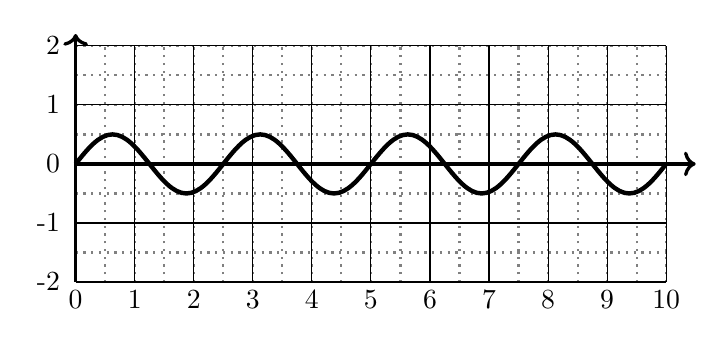
\begin{tikzpicture}[scale=0.75]
    \def\wl{2.5}
    \def\amp{0.5}
    \def\ymax{2}
    \def\xmax{10}
    \draw[dotted,thick,gray] 
      (0,-\ymax*1cm) grid[step=0.5cm] (\xmax*1cm,\ymax*1cm);
    \draw 
      (0,-\ymax*1cm) grid[step=1cm] (\xmax*1cm,\ymax*1cm);
    \foreach \x in {0,...,\xmax}{
      \draw (\x*1cm,-\ymax*1cm) ++(0,-.3cm) node {\x};
    }
    \foreach \y in {-\ymax,...,\ymax}{
      \node[anchor=east] at (-0.1cm,\y*1cm) {\y};
    }
    \draw[very thick,->] 
      (0,0) -- (\xmax*1cm,0) -- ++(0.5cm,0);
    \draw[very thick,->] 
      (0,-\ymax*1cm) -- (0,\ymax*1cm) -- ++(0,0.2cm);

    \draw[ultra thick] (0,0) 
      sin (0.25*\wl, \amp) cos (0.5*\wl, 0) 
      sin (0.75*\wl,-\amp) cos (    \wl, 0)
      sin (1.25*\wl, \amp) cos (1.5*\wl, 0)
      sin (1.75*\wl,-\amp) cos (2.0*\wl, 0)
      sin (2.25*\wl, \amp) cos (2.5*\wl, 0)
      sin (2.75*\wl,-\amp) cos (3.0*\wl, 0)
      sin (3.25*\wl, \amp) cos (3.5*\wl, 0)
      sin (3.75*\wl,-\amp) cos (4.0*\wl, 0);
  \end{tikzpicture}

  \begin{parts}
    \part 
      What kind of wave is this?

      \begin{solution}[\stretch{1}]
        transverse
      \end{solution}

    \part 
      What is its amplitude?
      
      \begin{solution}[\stretch{1}]
        0.5 m
      \end{solution}
      
    \part 
      What is the wavelength?
      
      \begin{solution}[\stretch{1}]
        2.5 m
      \end{solution}
      
    \part 
      What is the frequency?
      
      \begin{solution}[\stretch{1}]
        \begin{align*}
          v  &= f \lambda \\
          13 &= f (2.5) \\
          \SI{5.2}{\hertz} &= f
        \end{align*}
      \end{solution}
      

  \end{parts}



\end{questions}

\end{document}